% !TeX encoding=unicode
% !TeX spellcheck = de-DE

\chapter{Grundlagen}
\section{Next-to-leading order calculations}
\label{sec:nlo_calculations}
\ldots(need real and virtual, both seperately divergent, need to regularize)


There are two general methods that are commonly used to take care of the infrared divergences in NLO calculations, namely the \textit{slicing method} and the \textit{subtraction method}.
We can demonstrate both methods with a simple example similar to the depiction in \cite{slicing_vs_subtraction}.
Consider the integral
%
\begin{equation}
	I = \lim_{\epsilon \rightarrow 0} \left( \int_0^1 \frac{\dif x}{x} x^\epsilon F(x) - \frac{1}{\epsilon} F(0) \right) \, ,
\end{equation}
%
where $F(x)$ is an arbitrary function that depends on $x$.
The first term contains a singularity at $x=0$ and is divergent in the limit $\epsilon \rightarrow 0$.
This divergence is canceled by the second term.
The parameter $\epsilon$ can be compared to the parameter used in dimensional regularization.
As a consequence of $F(x)$ being arbitrary complex, the integral can not be solved analytically.
However, in this form it is also not well-suited for a numerical evalution because of the presence of $\epsilon$ in the integrand.

In the slicing method, one introduces a small parameter $\delta$, which slices the integration region into two pieces, so that the integral can be written in the following way:
%
\begin{align}
	I 	&= \lim_{\epsilon \rightarrow 0} \left( \int_0^\delta \frac{\dif x}{x} x^\epsilon F(x) + \int_\delta^1 \frac{\dif x}{x} x^\epsilon F(x) - \frac{1}{\epsilon} F(0) \right) \nonumber \\
		&= \lim_{\epsilon \rightarrow 0} \left( F(0) \int_0^\delta \frac{\dif x}{x} x^\epsilon - \frac{1}{\epsilon} F(0) \right) + \int_\delta^1 \frac{\dif x}{x} F(x) + \order{\delta} \nonumber \\
		&= F(0) \lim_{\epsilon \rightarrow 0} \frac{\delta^\epsilon - 1}{\epsilon} + \int_\delta^1 \frac{\dif x}{x} F(x) + \order{\delta} \nonumber \\
		&= F(0) \ln \delta + \int_\delta^1 \frac{\dif x}{x} F(x) + \order{\delta} \, .
\end{align}
%
Therefore, the dependence on $\epsilon$ has vanished completely and the remaining integral can be computed numerically.
The terms $\order{\delta}$ are neglectable if $\delta$ is small.
In an actual calculation, one would have to check that the result does not depend on the choice of $\delta$.

The subtraction method does not involve any approximations.
Instead, one rewrites the integral in the form
%
\begin{align}
	I	&= \lim_{\epsilon \rightarrow 0} \left( \int_0^1 \frac{\dif x}{x} x^\epsilon [F(x) - F(0)] + F(0) \int_0^1 \frac{\dif x}{x} x^\epsilon - \frac{1}{\epsilon} F(0) \right) \nonumber \\
		&= \int_0^1 \frac{\dif x}{x} [F(x) - F(0)] \, ,
\end{align}
%
which automatically leads to a form that can be evaluated by a numerical integration algorithm.
We can take a look at how this method works in a somewhat more realistic calculation.
Consider the expression for the expectation value of an infrared-safe observable $O$ at NLO accuracy, consisting of a Born (B), a virtual (V) und a real (R) term:
%
\begin{equation}
	\left< O \right> = \lim_{\epsilon \rightarrow 0} \int_0^1 \dif x x^{-2 \epsilon} O(x) \left[ \left( \od{\sigma}{x} \right)_B + \left( \od{\sigma}{x} \right)_V + \left( \od{\sigma}{x} \right)_R \right] \, .
\end{equation}
%
We assume that the cross sections can be written as
%
\begin{align}
	\left( \od{\sigma}{x} \right)_B &= B \delta(x) \, , \\
	\left( \od{\sigma}{x} \right)_V &= a \left( \frac{B}{2 \epsilon} + V \right) \delta(x) \, , \\
	\left( \od{\sigma}{x} \right)_R &= a \frac{R(x)}{x} \,
\end{align}
%
where $B$ and $V$ are constant factors and $\lim_{x \rightarrow 0} R(x) = B$.
$a$ denotes the coupling constant.
This model has been adapted from \cite{mcatnlo}.
Obviously, both the real and the virtual part are divergent in the limit $\epsilon \rightarrow 0$.
Using the subtraction method analogous to the case above, we can rewrite the real contribution to obtain
%
\begin{align}
	\left< O \right>_R	&= a \lim_{\epsilon \rightarrow 0} \int_0^1 \frac{\dif x}{x^{1+2 \epsilon}} O(x) R(x) \nonumber \\
						&= a B O(0) \lim_{\epsilon \rightarrow 0} \int_0^1 \frac{\dif x}{x^{1+2 \epsilon}} + a \int_0^1 \frac{\dif x}{x} [O(x) R(x) - B O(0)] \nonumber \\
						&= -a B O(0) \lim_{\epsilon \rightarrow 0} \frac{1}{2 \epsilon} + a \int_0^1 \frac{\dif x}{x} [O(x) R(x) - B O(0)] \, .
	\label{eq:toymodel_realsub}
\end{align}
%
By explicitely writing down the virtual part,
%
\begin{equation}
	\left< o \right>_V = a \lim_{\epsilon \rightarrow 0} \int_0^1 \frac{\dif x}{x^{2 \epsilon}} O(x) \left( \frac{B}{2 \epsilon} + V \right) \delta(x) \, ,
\end{equation}
%
we see that the first term gets exactly cancelled by the first term on the right hand side of \eqref{eq:toymodel_realsub}.
Including the Born contribtion we arrive at the expression
%
\begin{equation}
	\left< O \right> = B O(0) + a \left\{ V O(0) + \int_0^1 \frac{\dif x}{x} [O(x) R(x) - B O(0)] \right\} \, ,
\end{equation}
%
which now only consists of finite terms.

The subtraction method can be generalized to arbitrary hadronic cross sections, provided that the definition of the observables allows the cancellation of the divergences.
In simplified terms, it always leads to an expression of the form
%
\begin{equation}
	\sigma^\text{NLO}_{pp \rightarrow X} = \int \dif \hat \sigma^B + \int \dif \hat \sigma^V + \int \dif \hat \sigma^I + \int \dif \hat \sigma^{RS} \,
\end{equation}
%
consisting of a Born (B), a virtual (V), an integrated subtraction (I) and a real subtracted (RS) term.
All of these terms are seperately finite.
%
\section{Reweighting QCD calculations}
Often it is needed to vary the parameters in QCD calculations, for example the scale variables and PDFs to estimate the uncertainty.
When the number of variations becomes large, it is not practical to rerun the whole event generation for each calculation as the time and resource consumption become too high.
Instead it is possible to reuse information from previously generated events and combine them with the new parameters.
For a leading order calculation, this is straightforward:
Consider the leading order parton model cross section for producing an arbitrary final state X:
%
\begin{equation}
	\sigma_{pp \rightarrow X} = \sum_{i,j} \int \dif x_1 \dif x_2 \int \dif \Phi_n \left( \frac{\alpha_s(\mu_R^2)}{2 \pi} \right)^{p_\text{LO}} \pdf_i(x_1,\mu_F^2) \pdf_j(x_2,\mu_F^2) \dif \hat\sigma_{ij \rightarrow X} \, .
\end{equation}
%
The squared matrix element for the parton-level subprocess $2 \rightarrow n$ is denoted by $\dif \hat\sigma_{ij \rightarrow X}$, differential in the phase space $\dif \Phi_n$.
We can group subprocesses $s$ with the same parton-level cross section into a cumulated parton density $\subpdf_s(x_1,x_2,\mu_F^2)$ and write 
%
\begin{equation}
	\sigma_{pp \rightarrow X} = \int \dif x_1 \dif x_2 \int \dif \Phi_n \left( \frac{\alpha_s(\mu_R^2)}{2 \pi} \right)^{p_\text{LO}} \subpdf_s(x_1,x_2,\mu_F^2) \dif \hat\sigma_{ij \rightarrow X} \, .
\end{equation}
%
Rewriting this in a form that can be computed by a Monte Carlo algorithm on a per-event basis, we arrive at
%
\begin{equation}
  \sigma_{pp \rightarrow X} = \sum_{e=1}^{N_\text{evt}} \left( \frac{\alpha_s(\mu_R^2)}{2 \pi} \right)^{p_\text{LO}} w_e(k_e) \subpdf_{s_e}(x_1,x_2,\mu_F^2) \, .
  \label{eq:reweight_lo}
\end{equation}
%
The event weight $w_e(k_e)$ is given by
%
\begin{equation}
 	w_e(k_e) = \Pi_\text{ps}(k_e) \Theta(k_e - k_\text{cuts}) \dif \hat\sigma_e
\end{equation}
%
and represents the subprocess cross section $\dif \hat\sigma_e$ with respect to the phase space weight $\Pi_\text{ps}(k_e)$ and the kinematic cuts.
The kinematic parameters for each event are combined in
%
\begin{equation}
  k_e = \left\{ p_1 , \dots , p_n , x_1 , x_2 \right\} \, ,
\end{equation}
%
where the $p_i$ denote the involved partons.

Provided that all event weights have been stored, using a different PDF is as simple as multiplying each weight with the new PDF $\subpdf^\text{new}_{s_e}(x_1,x_2,\mu_F^2)$.
The value of $\alpha_s$ can be changed similarly.
To vary the scales, only $\alpha_s$ and $\subpdf_{s_e}$ have to be reevaluated as the weights themselves do not depend on the scales.

At NLO the reweighting becomes more involved.
The event weights now depend explicitely on the scales and due to the appearance of divergences in the calculaion of the parton-level cross sections, a method for cancelling these divergences has to be used.
In the following, we will examine the method used by \mcgrid{} to reweight NLO calculations.
It expects, that the events are generated using the Catani-Seymour dipole subtraction method \cite{catani_seymour1997}, which is a general algorithm for the automatic calculation of arbitrary jet cross sections at NLO.
It is based on the subtraction method introduced in \secref{sec:nlo_calculations}.

As we have seen, the subtraction method splits the calculation into four parts: The Born (B), virtual (V), integrated subtraction (I) and real subtraction (RS) part.
All of these have to be handled differently.
How this is done in detail can be seen in the original \mcgrid{} paper \cite{mcgrid2013}.
The important result is, that if we treat the different contributions as single events, the NLO result can be written in a form similar to the LO expression \eqref{eq:reweight_lo}:
%
\begin{equation}
  \sigma^\text{NLO}_{pp \rightarrow X} = \sum_{e=1}^{N_\text{evt}} \left( \frac{\alpha_s(\mu_R^2)}{2 \pi} \right)^{p_e} w_e(k_e) \subpdf_{s_e}(x_1,x_2,\mu_F^2) \, ,
  \label{eq:reweight_nlo}
\end{equation}
%
where $p_e$ is the order in $\alpha_s$ of the respective event, i.e.\ $p_e = p_\text{LO}$ for B events and $p_e = p_\text{LO} + 1$ for I, V and RS events.
This allows for simple \textit{a posteriori} parameter variation analogous to the LO case.
%
\section{The considered process: Higgs production through gluon fusion}
In this thesis, the considered process will be the production of a Higgs boson through gluon fusion.
Although there are other possible production mechanisms in the Standard Model, this is the main process at the LHC, with an expected cross section of $\approx \SI{50}{\pico\barn}$ at a center-of-mass energy of $\sqrt{s} = \SI{14}{\tera\electronvolt}$ and a Higgs mass of $\SI{125}{\giga\electronvolt}$. \cite{higgshandbook1}
It proceeds through a triangular loop of heavy quarks (mainly top quarks as the Higgs coupling scales with the quark mass) as is shown in \figref{fig:gluonfusion}
%
\begin{figure}[]
	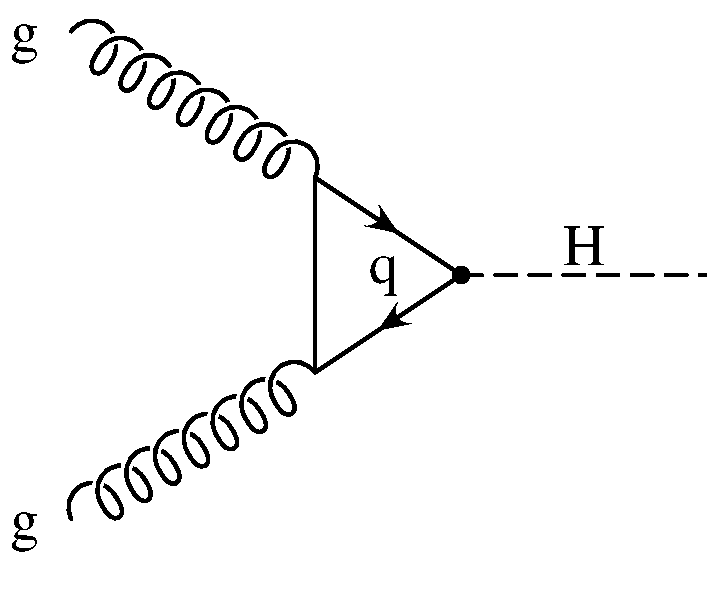
\includegraphics[width=0.5\textwidth]{images/gluonfusion.pdf}
	\caption{Higgs production through gluon fusion.}
	\label{fig:gluonfusion}
\end{figure}
%

In the narrow-width approximation, the leading order cross section is given by \cite{gluonfusioncrosssection}
%
\begin{equation}
	\sigma_\text{LO}(pp \rightarrow H) = \sigma_0^H \tau_H \od{\lumi^{gg}}{\tau_H} \, ,
\end{equation}
%
where $\tau_H = M_H^2/s$ is the Drell-Yan variable and $\dif \lumi^{gg} / \dif \tau_H$ is the gluon luminosity.
The partonic cross section $\sigma_0^H$ can be written as
\begin{equation}
	\sigma_0^H = \frac{G_F \alpha_s^2(\mu_R^2)}{288 \sqrt{2} \pi} \abs{ \sum_q \frac{3}{2 \tau_q} \left[ 1 + \left( 1 - \frac{1}{\tau_q} \right) f(\tau_q) \right] }^2  \, ,
\end{equation}
%
with the form factor
%
\[ f(\tau_q) = 
\begin{cases}
	\arcsin^2 \left( \sqrt{\tau_q} \right) ,																& \tau_q < 1, \\
	- \frac{1}{4} \left[ \ln \frac{1 + \sqrt{1-\tau_q^{-1}}}{1 - \sqrt{1-\tau_q^{-1}}} -i \pi \right]^2 ,	& \tau_q > 1,
\end{cases}
\]
%
where $G_F$ denotes the Fermi coupling constant and $\tau_q = m_H^2/4m_q^2$.
The gluon luminosity takes the form
%
\begin{equation}
	\od{\lumi^{gg}}{\tau_H} = \int_0^1 \dif x_1 \dif x_2 \gluonpdf(x_1,\mu_F^2) \gluonpdf(x_2,\mu_F^2) \delta(x_1 x_2 - \tau_q) \,
\end{equation}
%
with $\gluonpdf(x,\mu_F^2)$ denoting the gluon PDF.

The QCD corrections are composed of virtual corrections to the vertices and propagators, real gluon radiation in the initial state and the contributions of the subprocesses $gq \rightarrow Hq$ and $q \bar q \rightarrow Hg$.
Exemplary diagrams for the corrections are shown in \figref{fig:ggh_corrections}.

%
\begin{figure}
\centering
\begin{subfigure}[]{0.3\textwidth}
	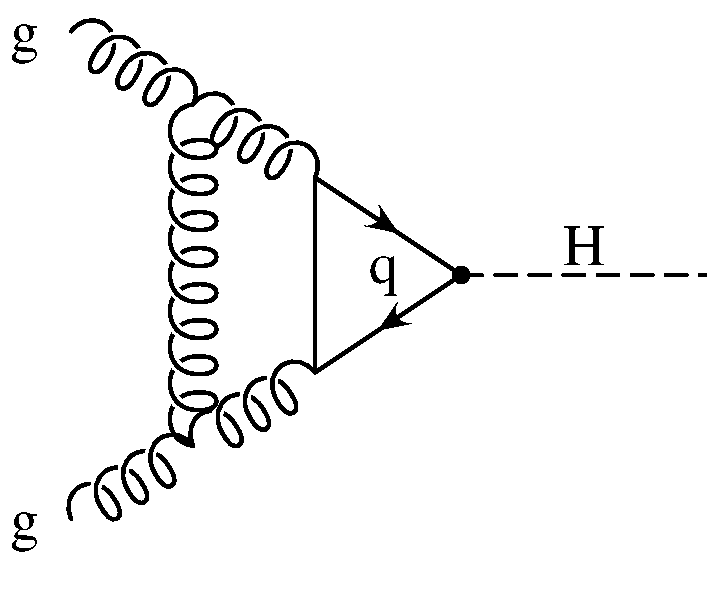
\includegraphics[width=\textwidth]{images/gluonfusion_virtual1.pdf}
	\caption{}
\end{subfigure}
~
\begin{subfigure}[]{0.3\textwidth}
	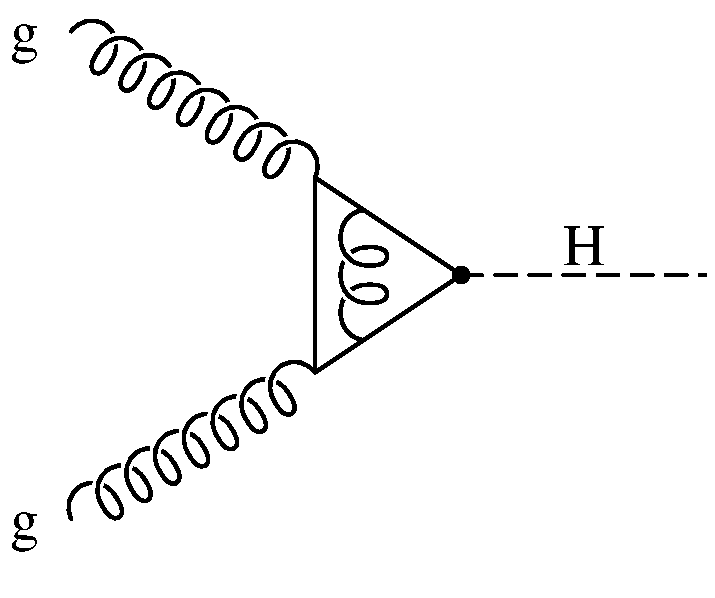
\includegraphics[width=\textwidth]{images/gluonfusion_virtual2.pdf}
	\caption{}
\end{subfigure}
~
\begin{subfigure}[]{0.3\textwidth}
	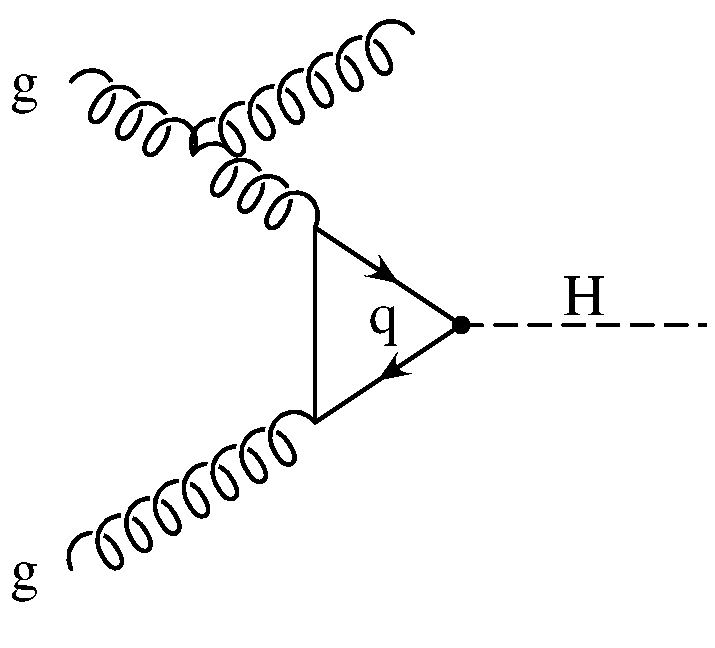
\includegraphics[width=\textwidth]{images/gluonfusion_real1.pdf}
	\caption{}
\end{subfigure}

\begin{subfigure}[]{0.3\textwidth}
	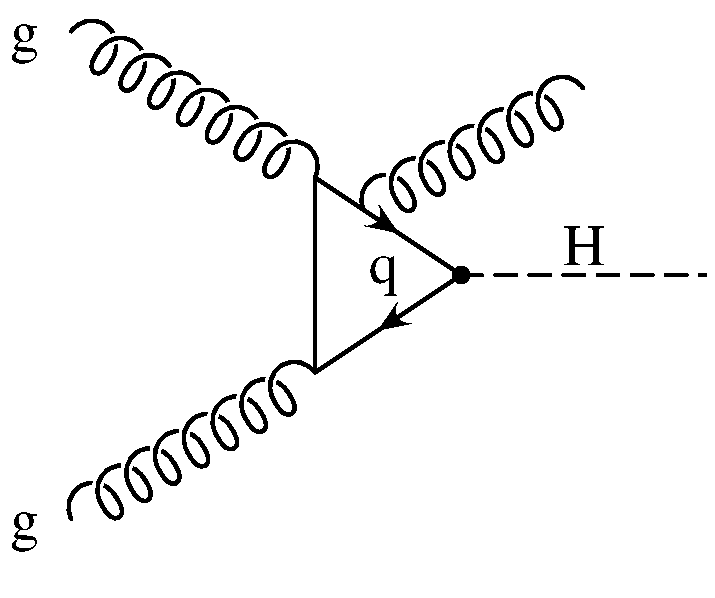
\includegraphics[width=\textwidth]{images/gluonfusion_real2.pdf}
	\caption{}
\end{subfigure}
~
\begin{subfigure}[]{0.3\textwidth}
	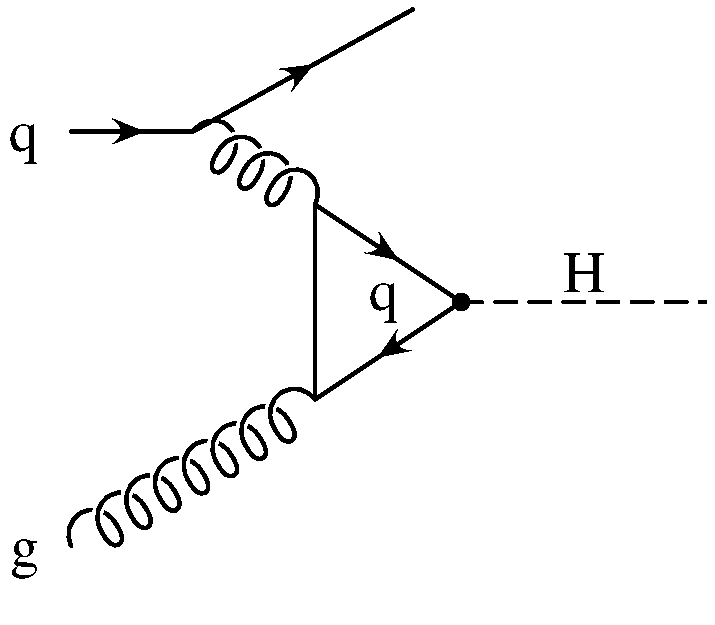
\includegraphics[width=\textwidth]{images/gq_hq.pdf}
	\caption{}
\end{subfigure}
~
\begin{subfigure}[]{0.3\textwidth}
	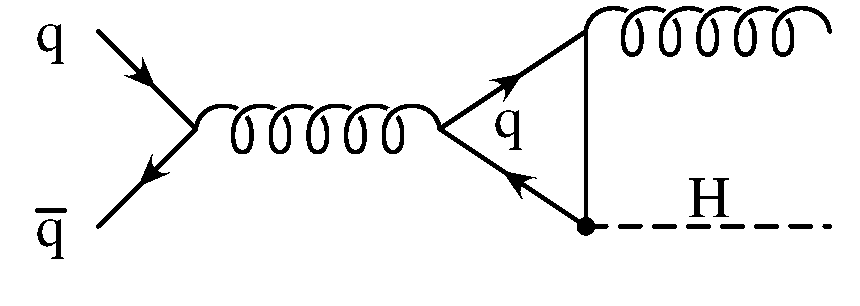
\includegraphics[width=\textwidth]{images/qq_hg.pdf}
	\caption{}
\end{subfigure}
\caption{Example diagrams illustrating the QCD corrections to the process $pp \rightarrow H$:
		(a), (b) virtual corrections; (c), (d) real emission of a gluon; (e) $gq \rightarrow Hq$; (f) $q \bar q \rightarrow Hg$.}
\label{fig:ggh_corrections}
\end{figure}
%

The NLO QCD corrections to the cross section have been calculated in \cite{gfusionnlo1}.
They increase the cross section by a factor of \num{1.5} to \num{1.7}.
In the limit where the top quark has infinite mass, $m_t \rightarrow \infty$, the form factor takes the value $\frac{4}{3}$.
This allows for an analytical expression for the corrections \cite{gfusionnlo2}, which is very well suited for numerical calculations.
It can be considered as an extension of the Standard Model, where the Higgs boson couples directly to gluons (effective Higgs coupling).
In many cases, this is a rather good approximation \cite{symmetrybreaking1}.

The NNLO corrections have been calculated in \cite{gfusionnnlo1, gfusionnnlo2}.


A fully differential NNLO calculation exists for $H + 0-\text{jet}$ production \cite{ggh_nnlo_fullydiff_1,ggh_nnlo_fullydiff_2} and substantial progress has been achieved towards an NNLO calculation of the $1-\text{jet}$ cross section \cite{gghj_nnlo_progress}.
The fully differential NLO cross section is available for $H + 1-\text{jet}$ \cite{gghj_nlo_fullydiff_1,gghj_nlo_fullydiff_2}, $H + 2-\text{jets}$ \cite{gghjj_nlo_fullydiff_1,gghjj_nlo_fullydiff_2} and $H + 3-\text{jets}$ \cite{gghjjj_nlo_fullydiff}.


The effective Lagrangian for Higgs gluon interaction can be written as \cite{gfusionnnlo2}
%
\begin{equation}
	\Lagr_\text{eff}^{ggH} = - \frac{1}{4v} C_1 G_{\mu \nu}^a {G^a}^{\mu \nu} H \, ,
\end{equation}
%
where $v$ is the Higgs vacuum expectation value, $G^a_{\mu \nu}$ is the gluon field strength tensor and $H$ is the Higgs field.
The coefficient $C_1$, in the \msbar{} scheme, is given by
%
\begin{align}
	C_1 = \frac{-1}{3 \pi} &\left\{1 + \frac{11 \alpha_s}{4 \pi} + \left( \frac{\alpha_s}{\pi} \right)^2 \left[ \frac{2777}{288} + \frac{19}{16} \log\left( \frac{\mu^2}{m_t^2} \right)
	\vphantom{n_f \left( -\frac{67}{96} + \frac{1}{3} \log\left( \frac{\mu^2}{m_t^2} \right) \right)} \right. \right. \nonumber \\
	%	
		&\qquad \left. \left. \vphantom{\frac{2777}{288} + \frac{19}{16} \log\left( \frac{\mu^2}{m_t^2} \right)}
		+ n_f \left( -\frac{67}{96} + \frac{1}{3} \log\left( \frac{\mu^2}{m_t^2} \right) \right) \right] + \order{\alpha_s^3} \right\} \, ,
\end{align}
%
where the number of active flavors should be set to $n_f = 5$.
According to \cite{gfusionnnlo2}, at LO this approximation is accurate within \SI{5}{\percent} for $m_H \approx \SI{150}{\giga\electronvolt}$ (which is close to the measured value $m_H \approx \SI{126}{\giga\electronvolt}$) and improves at NLO.

\section{Leptonic Higgs decay}
There are several possible decay channels for the Higgs boson.
One has to keep in mind that the Higgs coupling is proportional to the particle masses, so that it will decay into the heaviest possible particles.
Assuming a Higgs mass of $m_H = \SI{126}{\giga\electronvolt}$, the most relevant decay products are $q \bar q$ (where q denotes a bottom or charm quark), $WW$, $ZZ$, $Z \gamma$, $\gamma \gamma$, $gg$ and $\tau^+ \tau^-$ \cite{higgshandbook2}.
The decay into photons or gluons is only possible through intermediate loops.

The studies leading to the discovery of the Higgs boson at the LHC relied primarily on the decay modes $H \rightarrow \gamma \gamma$, $H \rightarrow ZZ$ and $H \rightarrow WW$.

\ldots
For the purpose of this thesis, we will consider the decay $H \rightarrow \tau^+ \tau^-$, which has a branching ratio of approximately \SI{6}{\percent} \cite{higgshandbook3}.
\ldots
There have been searches for $H \rightarrow \tau \tau$ events in the LHC data and both ATLAS \cite{htau_atlas} and CMS \cite{htau_cms} have published evidences for this type of decay.
